\chapter{Frontend}
\section{Use-Cases}
\begin{figure}[h]
	\centering
	\label{design:dia:usecase}
	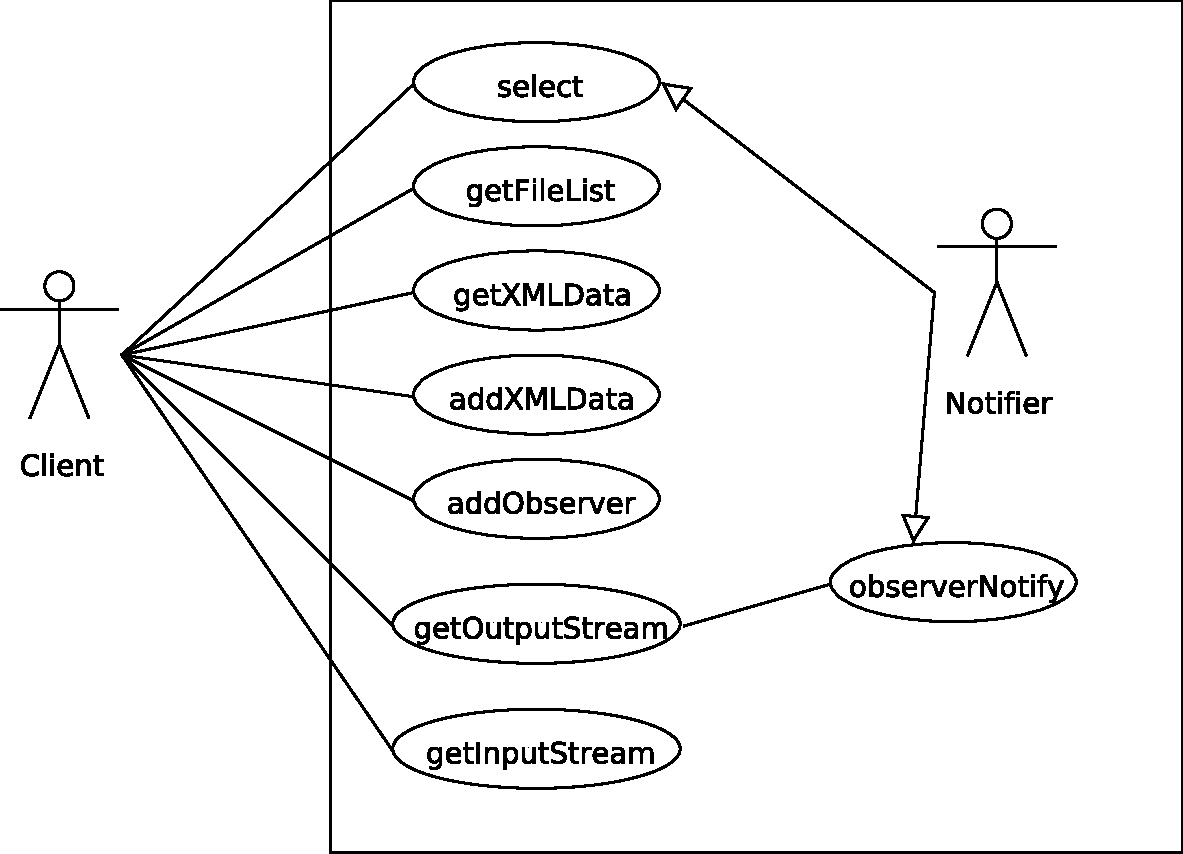
\includegraphics[width=\textwidth]{design/frontend/usecase-client.pdf}
	\caption{Diagramm: Use-Cases - Client und Server}
\end{figure}
\begin{description}
	\item [select]
	\item [getFileList]
	\item [getOutputStream]
	\item [getInputStream]
	\item [getXMLData]
	\item [addXMLData]
	\item [add / deleteObserver]
	\item [notifyClients]
\end{description}

\section{Schnittstellen und Api}

\section{Programmfluss}

\subsection {select}

\begin{figure}[h]
	\centering
	\label{design:dia:sqc:select}
	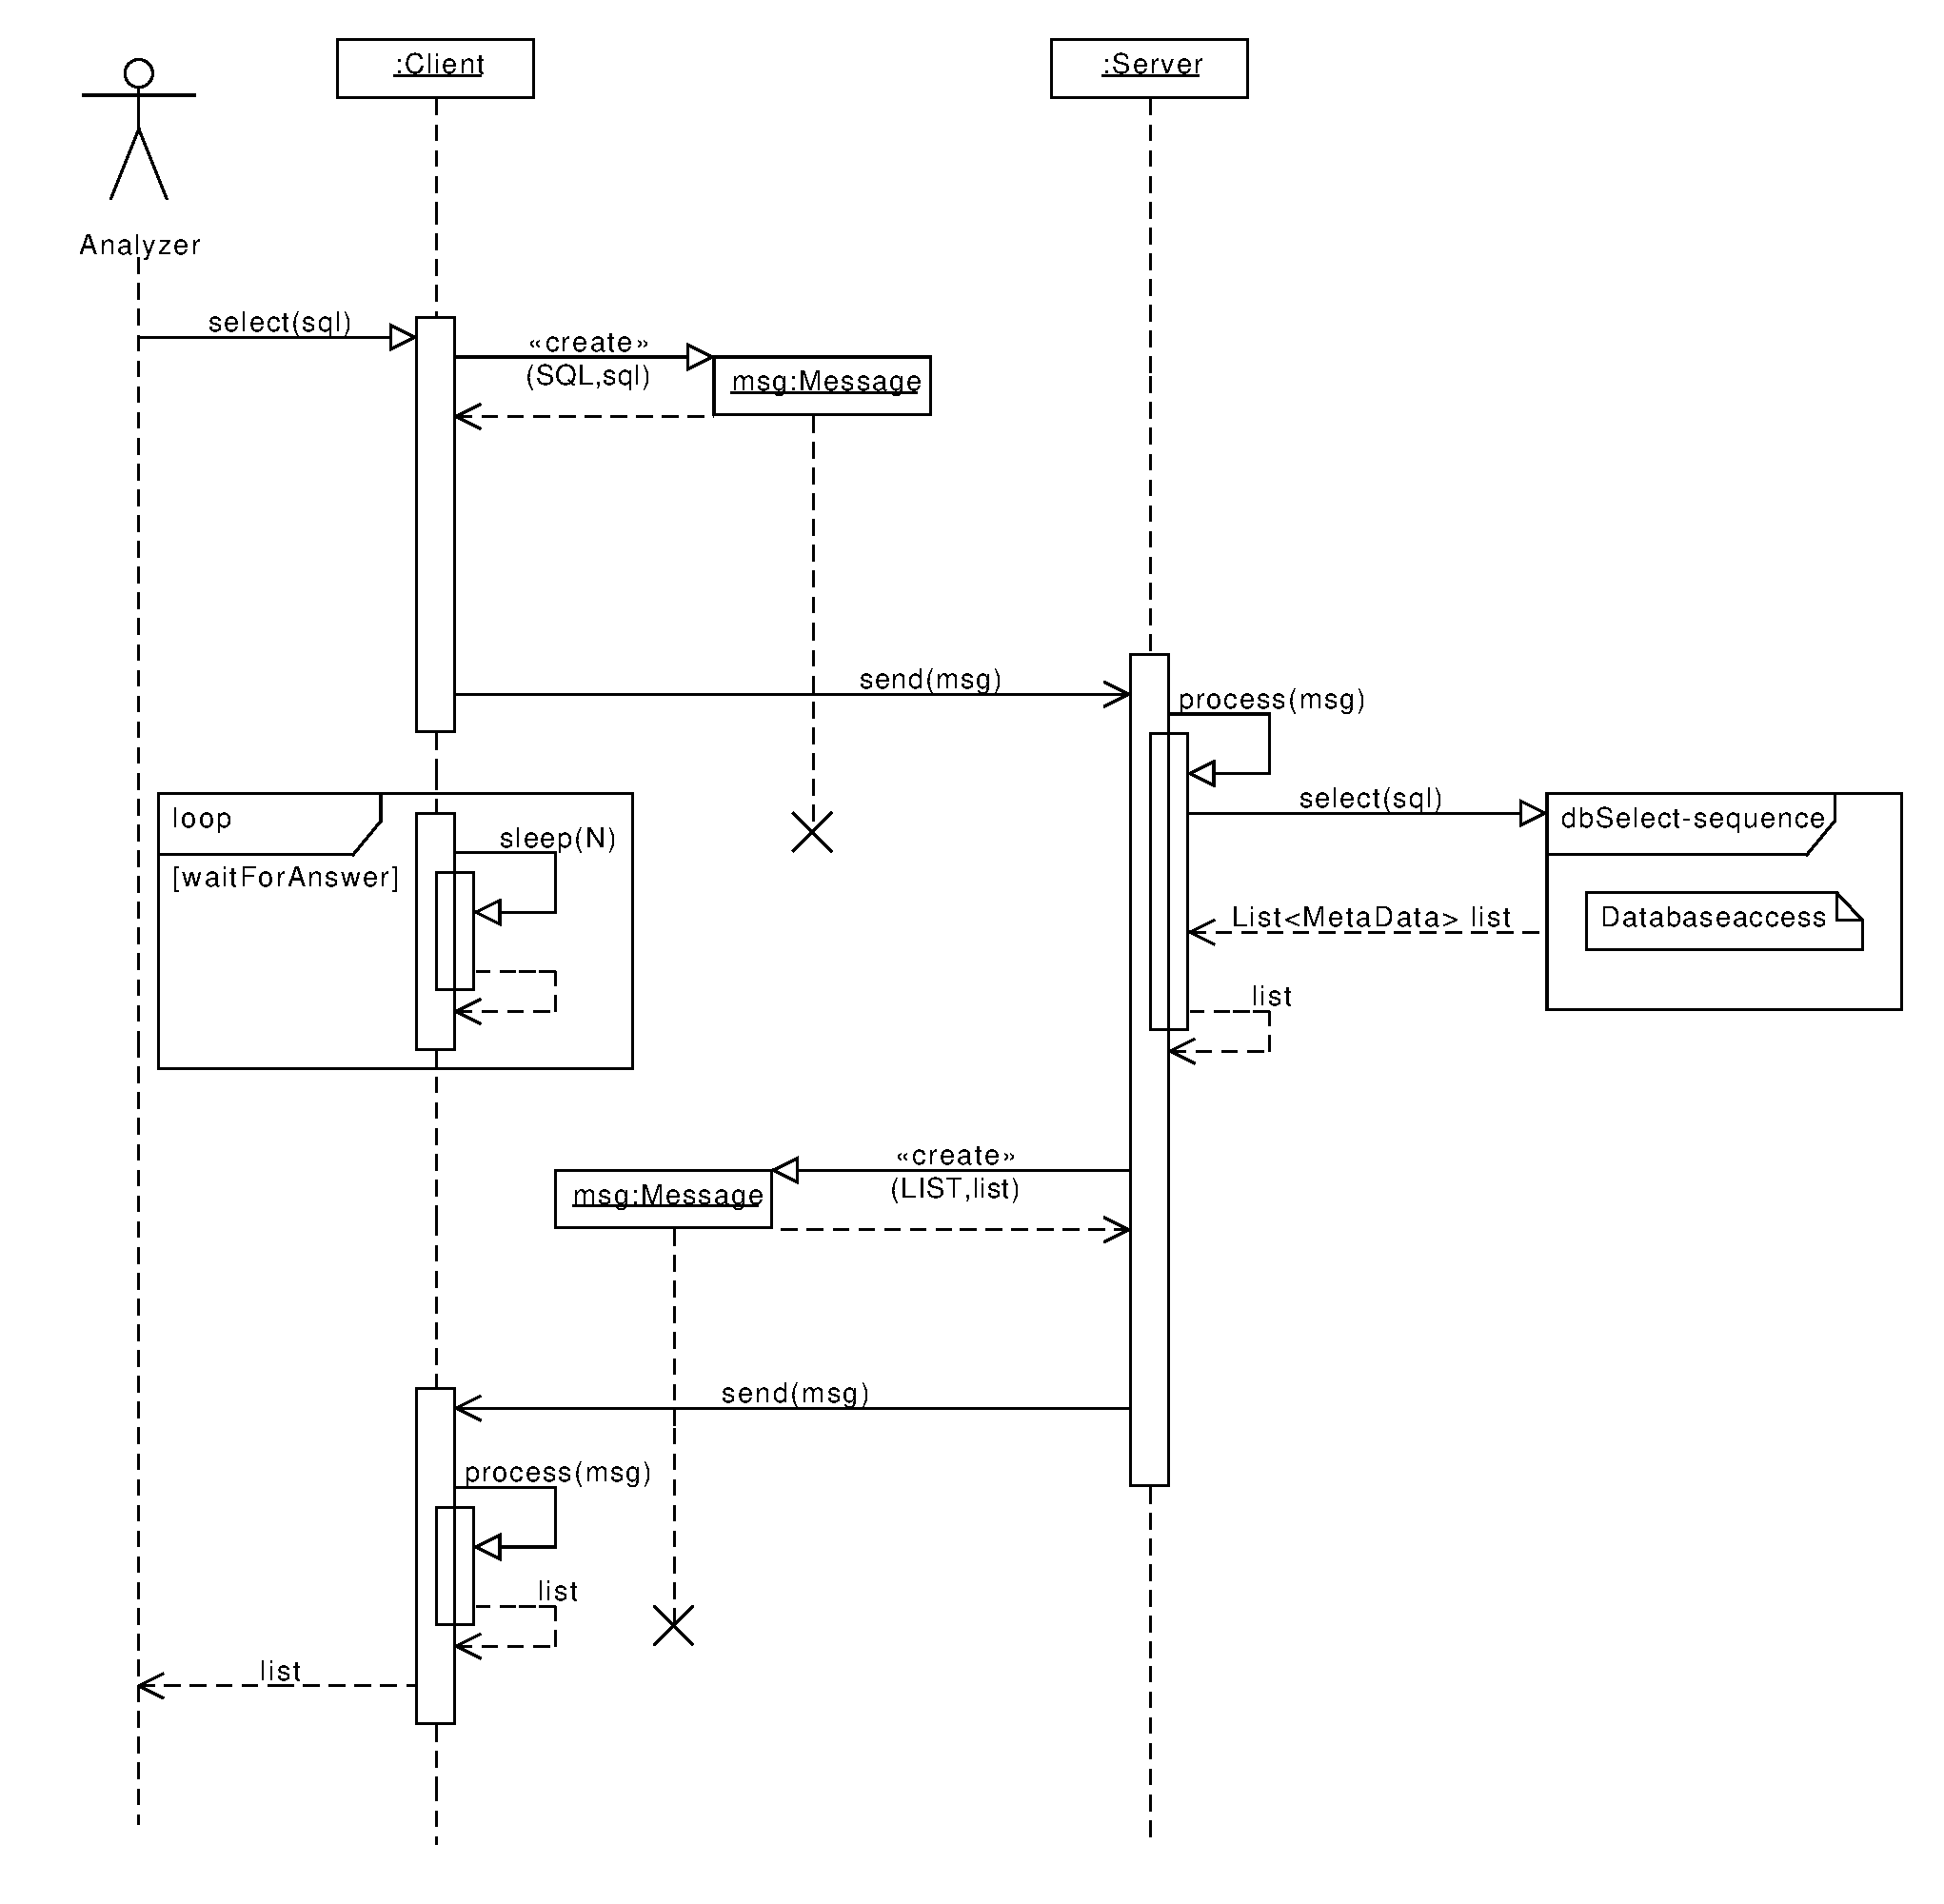
\includegraphics[width=\textwidth]{design/frontend/sequence/select-sequence.pdf}
	\caption{Sequenzdiagramm: Select}
\end{figure}

\subsection {getFileList}
\todo{sequence: getFileList}
%\begin{figure}[h]
%	\centering
%	\label{design:dia:sqc:select}
%	\includegraphics[width=\textwidth]{design/frontend/sequence/.pdf}
%	\caption{Sequenzdiagramm: Select}
%\end{figure}

\subsubsection{Lock setzen}
\begin{figure}[h]
	\centering
	\label{design:dia:sqc:lock}
	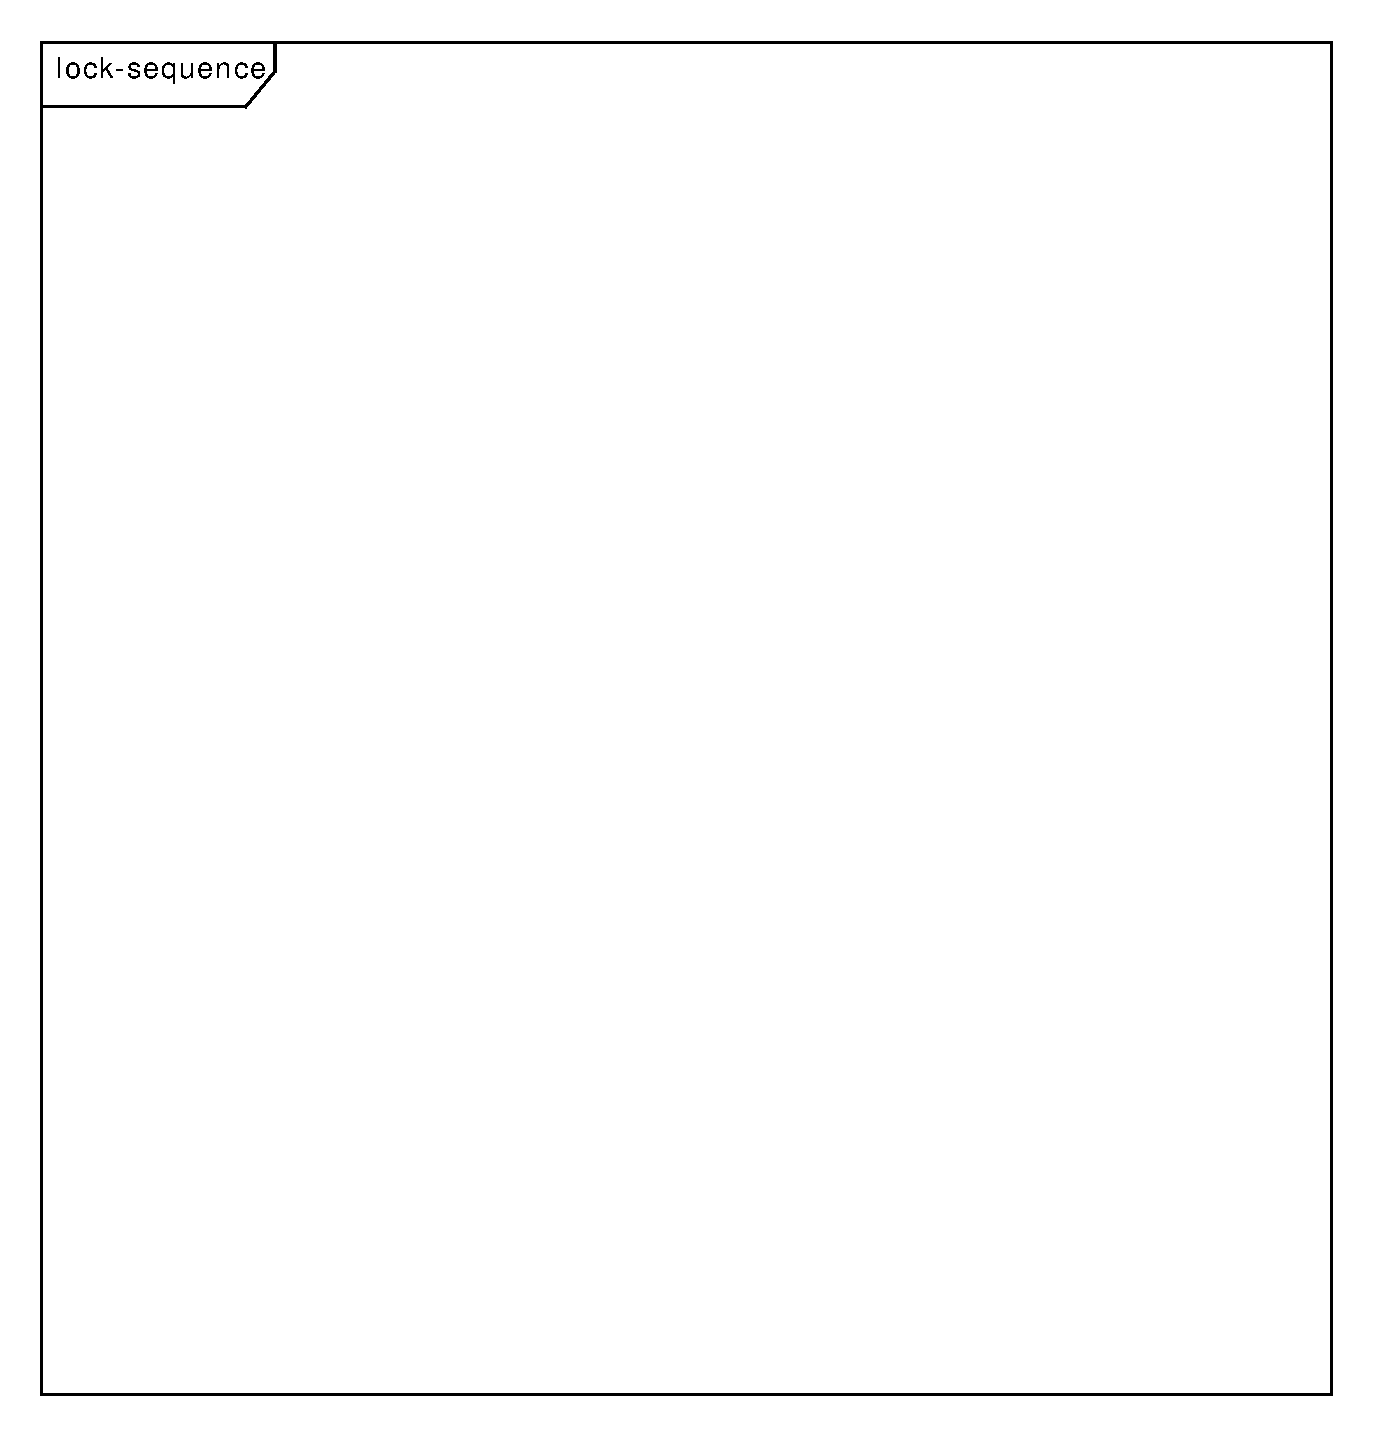
\includegraphics[width=\textwidth]{design/frontend/sequence/lock-sequence.pdf}
	\caption{Sequenzdiagramm: Lock setzen}
\end{figure}

\subsubsection{Unlock}
\begin{figure}[h]
	\centering
	\label{design:dia:sqc:unlock}
	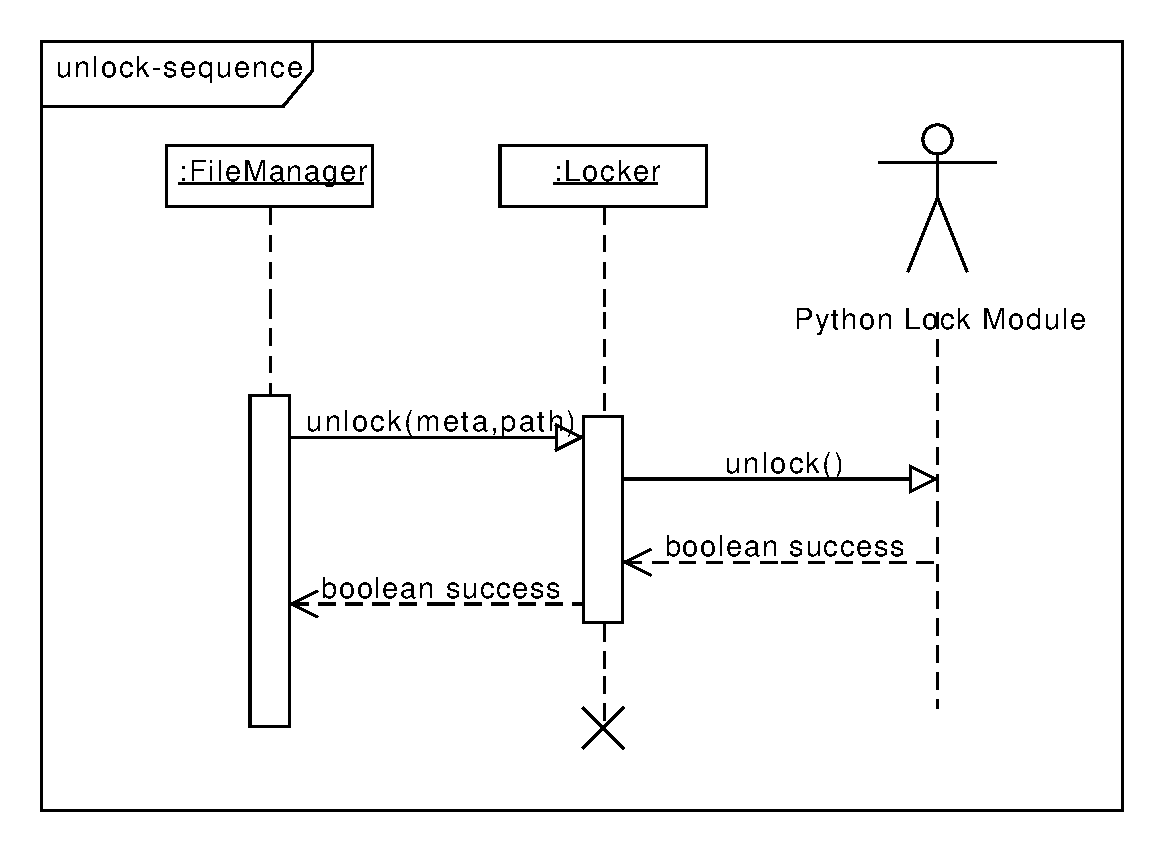
\includegraphics[width=\textwidth]{design/frontend/sequence/unlock-sequence.pdf}
	\caption{Sequenzdiagramm: Unlock}
\end{figure}

\subsection {getOutputStream}
\begin{figure}[h]
	\centering
	\label{design:dia:sqc:getOutputStream}
	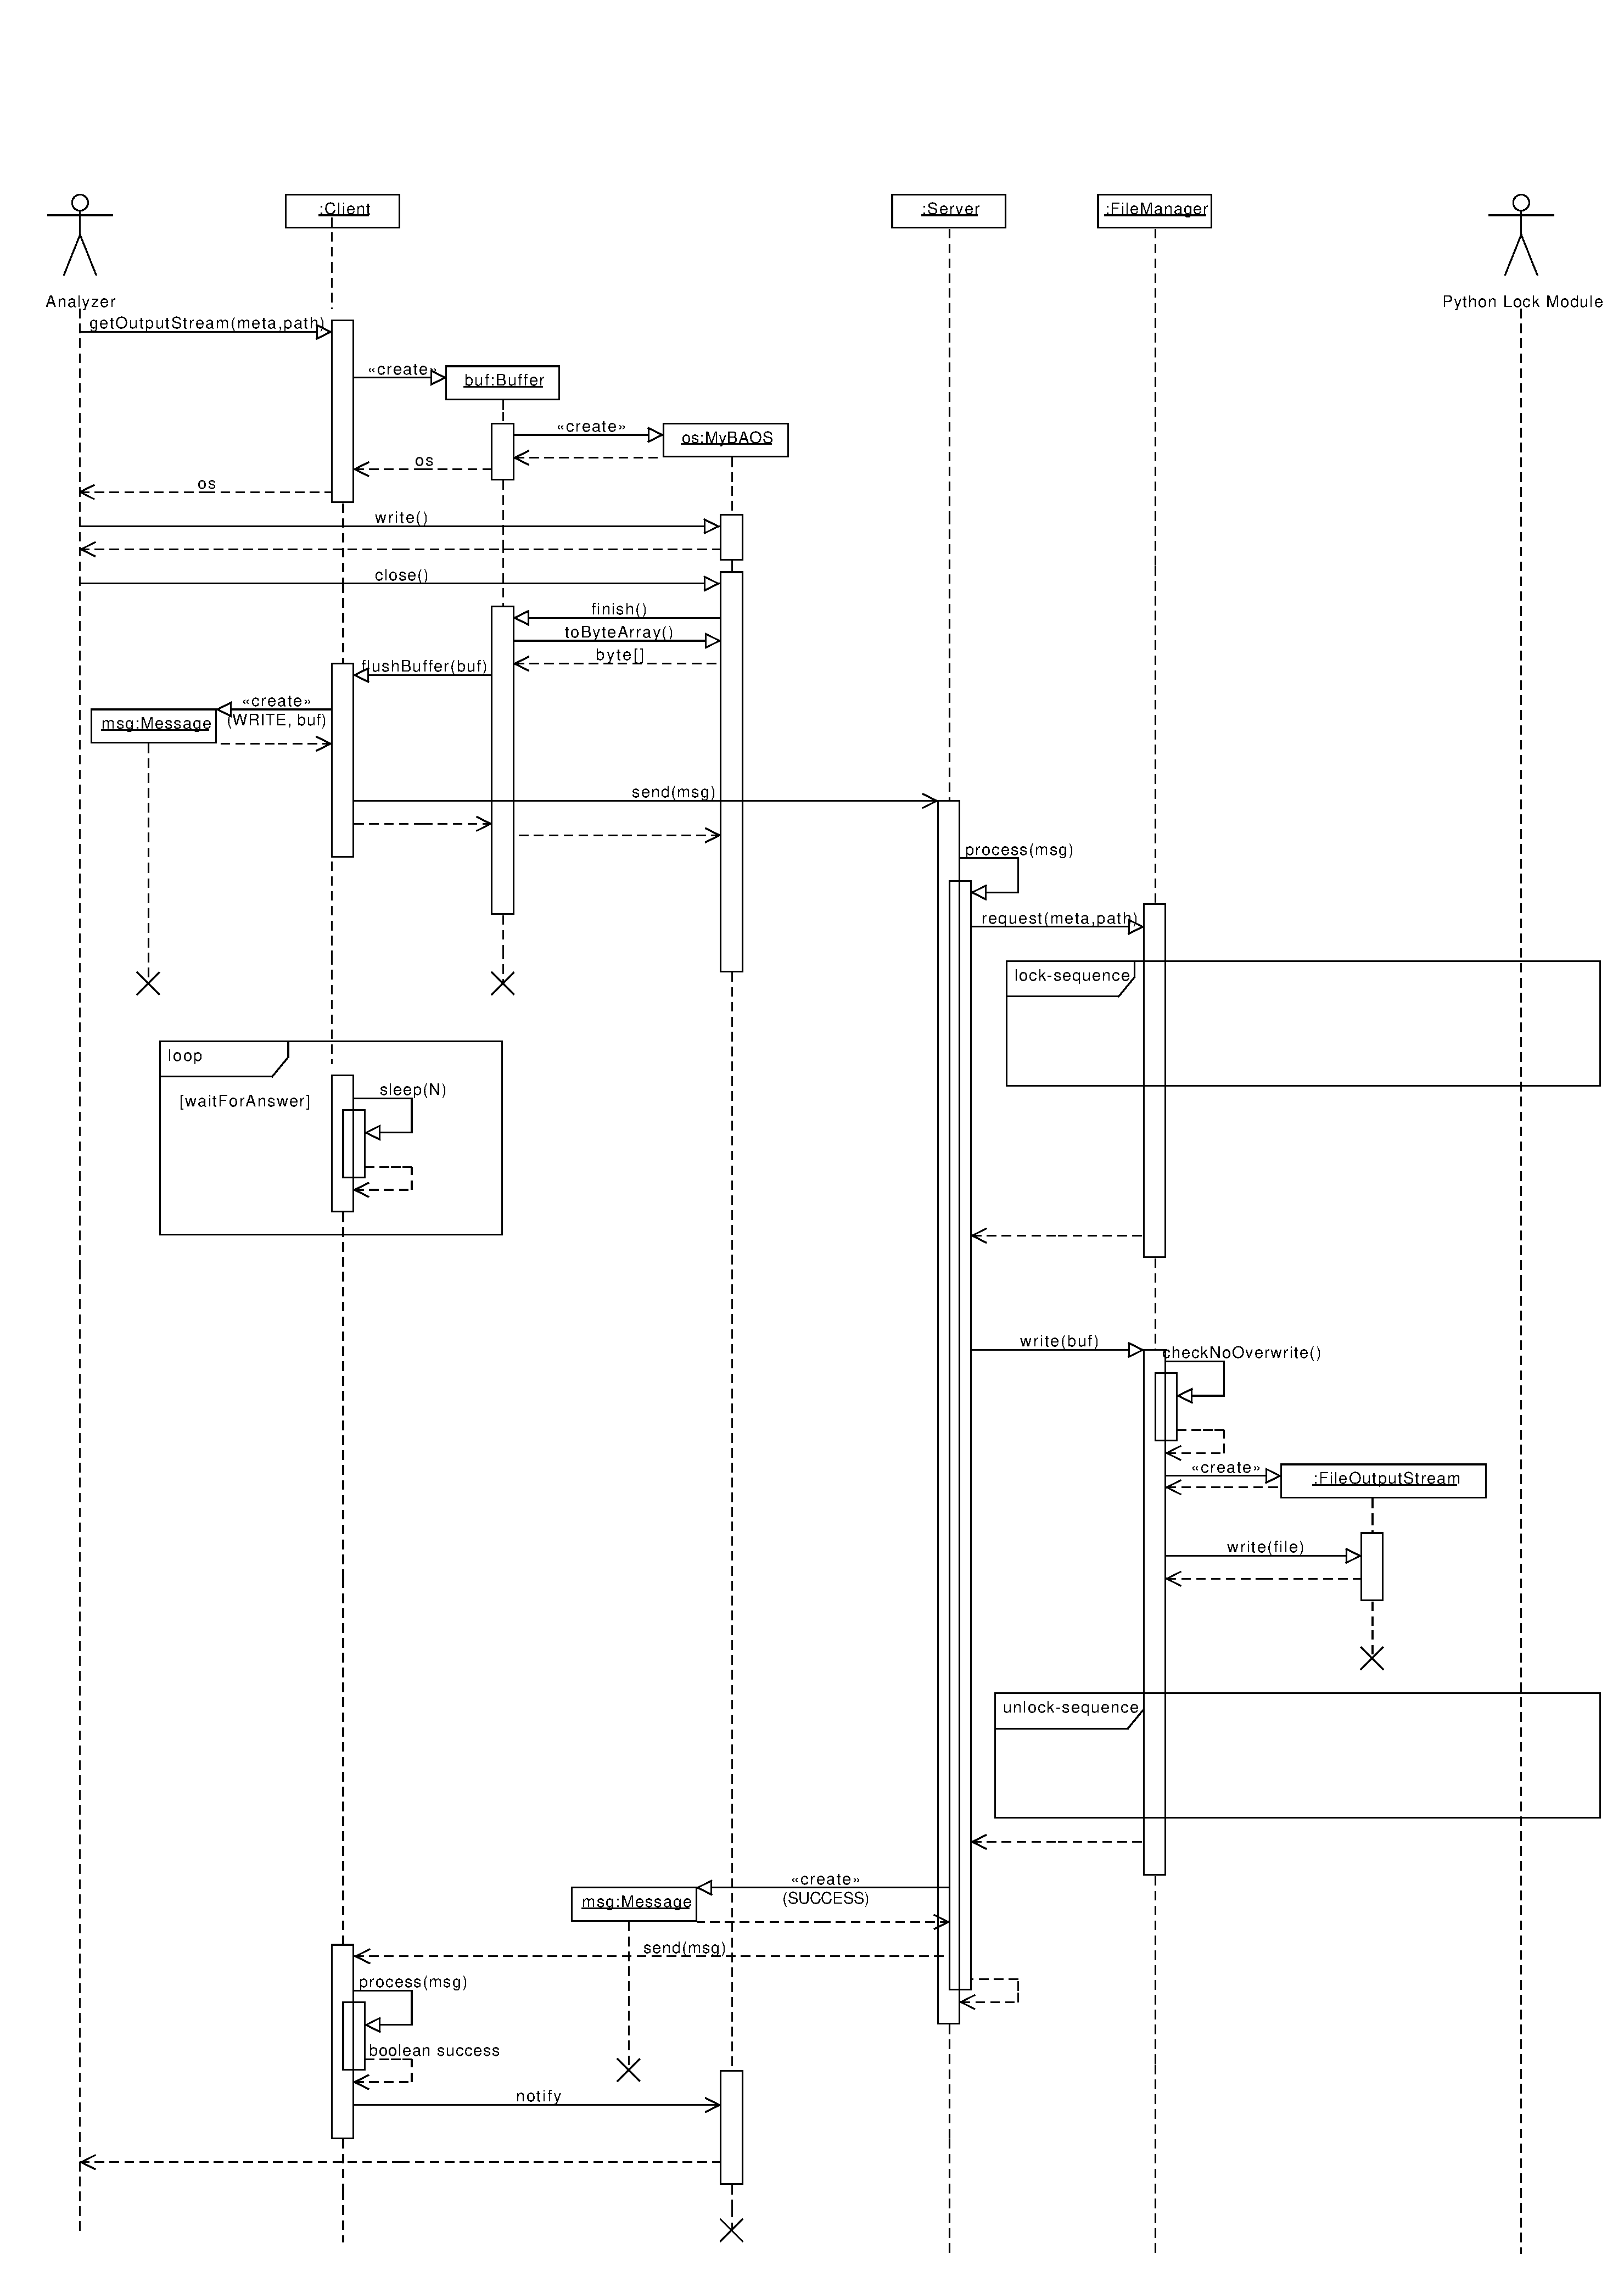
\includegraphics[width=\textwidth]{design/frontend/sequence/get-output-stream-sequence.pdf}
	\caption{Sequenzdiagramm: getOutputStream}
\end{figure}

\subsection {getInputStream}
\begin{figure}[h]
	\centering
	\label{design:dia:sqc:getInputStream}
	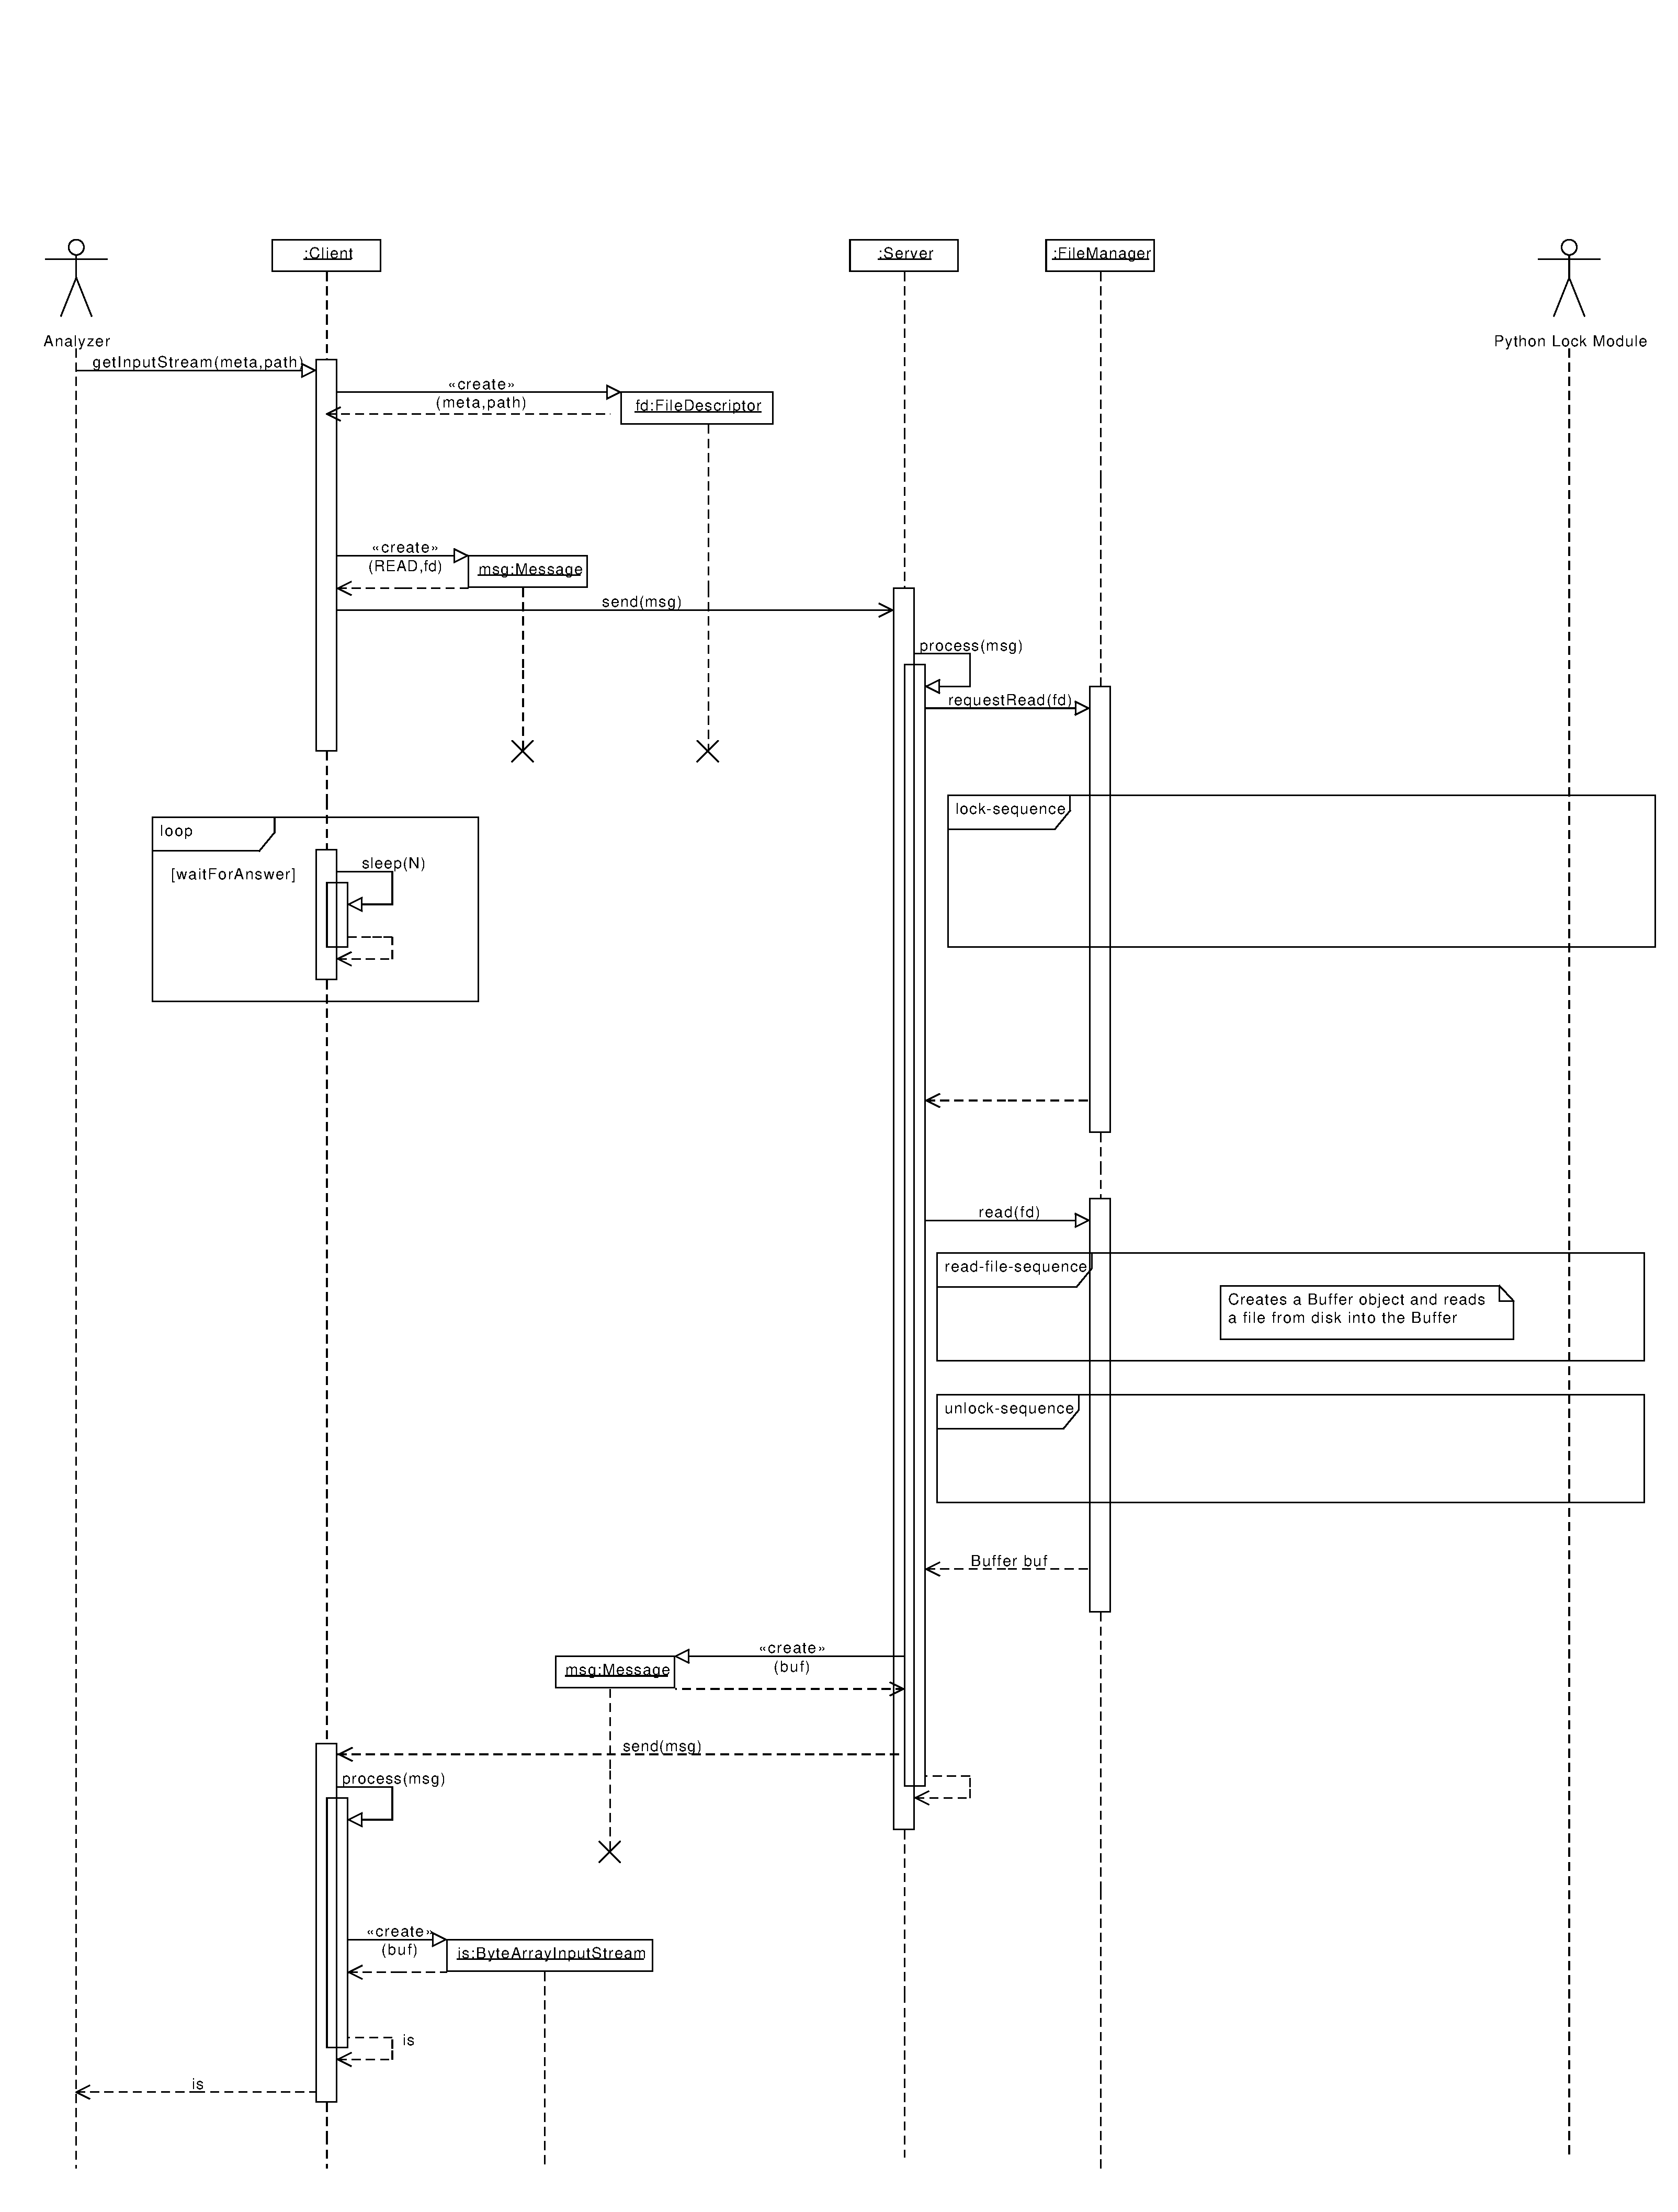
\includegraphics[width=\textwidth]{design/frontend/sequence/get-input-stream-sequence.pdf}
	\caption{Sequenzdiagramm: getInputStream}
\end{figure}

\subsection {getXMLData}
\todo{sequence: getXMLData}
%\begin{figure}[h]
%	\centering
%	\label{design:dia:sqc:select}
%	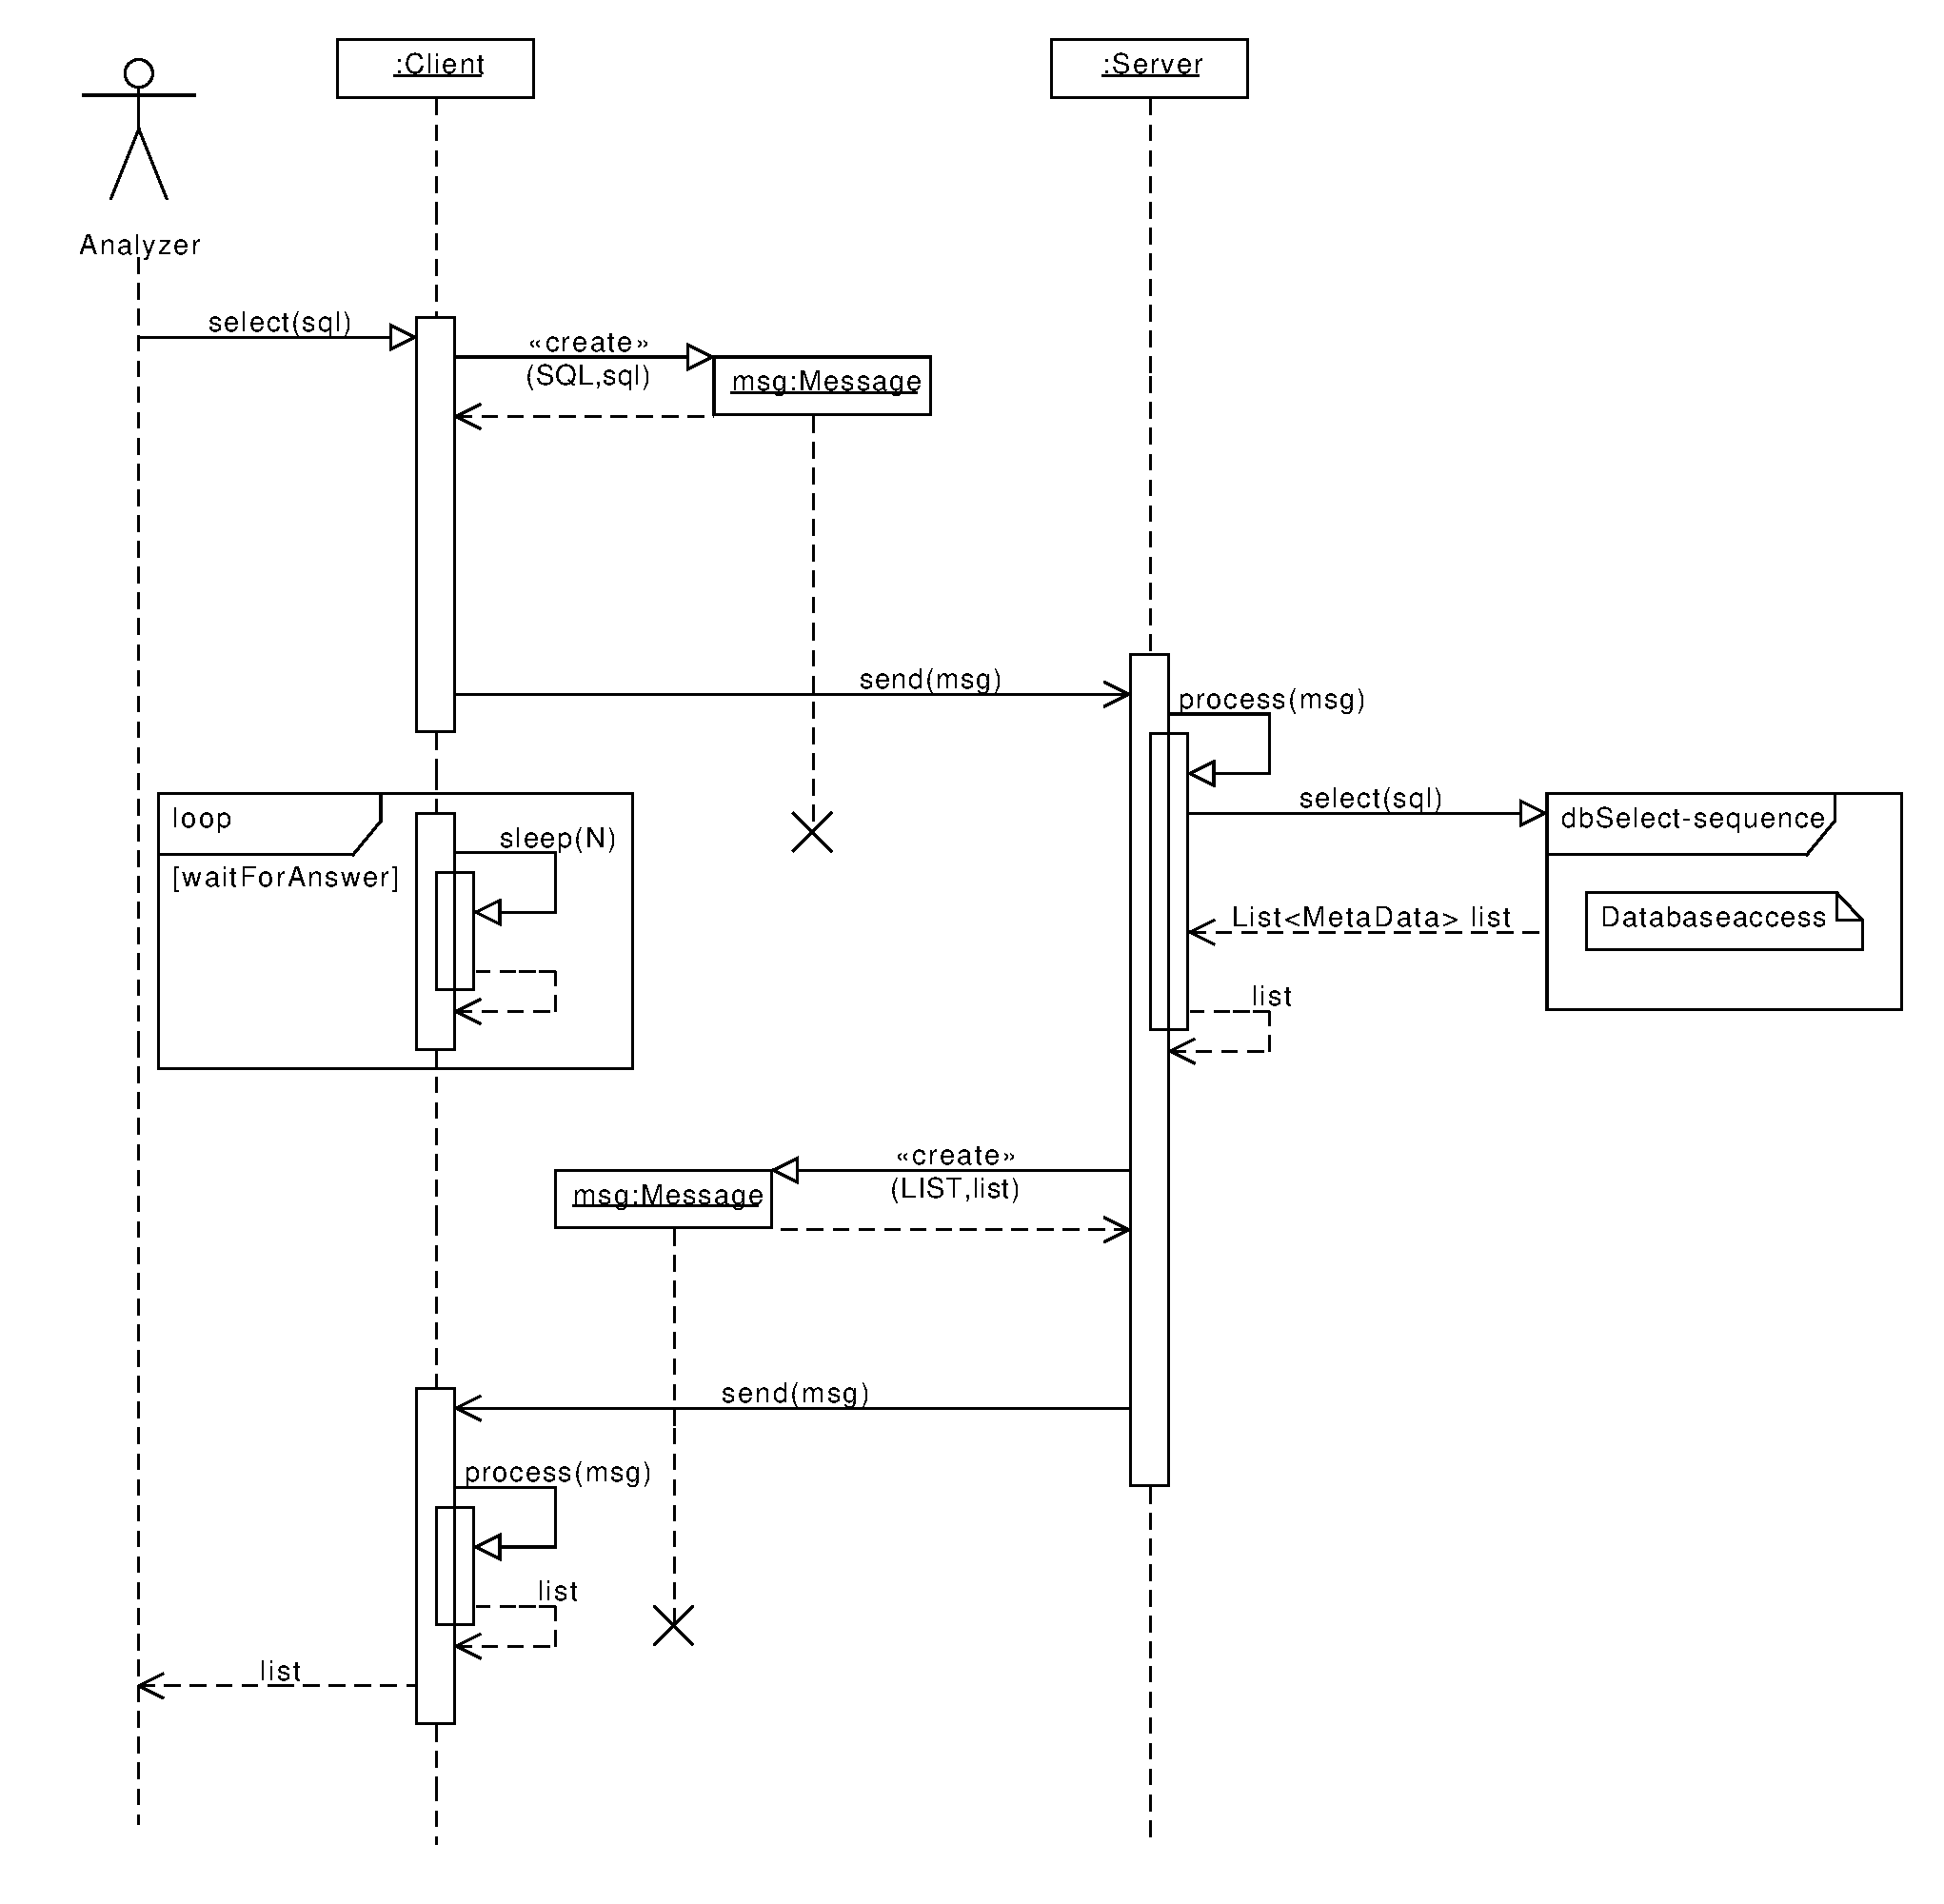
\includegraphics[width=\textwidth]{design/frontend/sequence/select-sequence.pdf}
%	\caption{Sequenzdiagramm: Select}
%\end{figure}

\subsection {addXMLData}
\todo{sequence: addXMLData}
%\begin{figure}[h]
%	\centering
%	\label{design:dia:sqc:select}
%	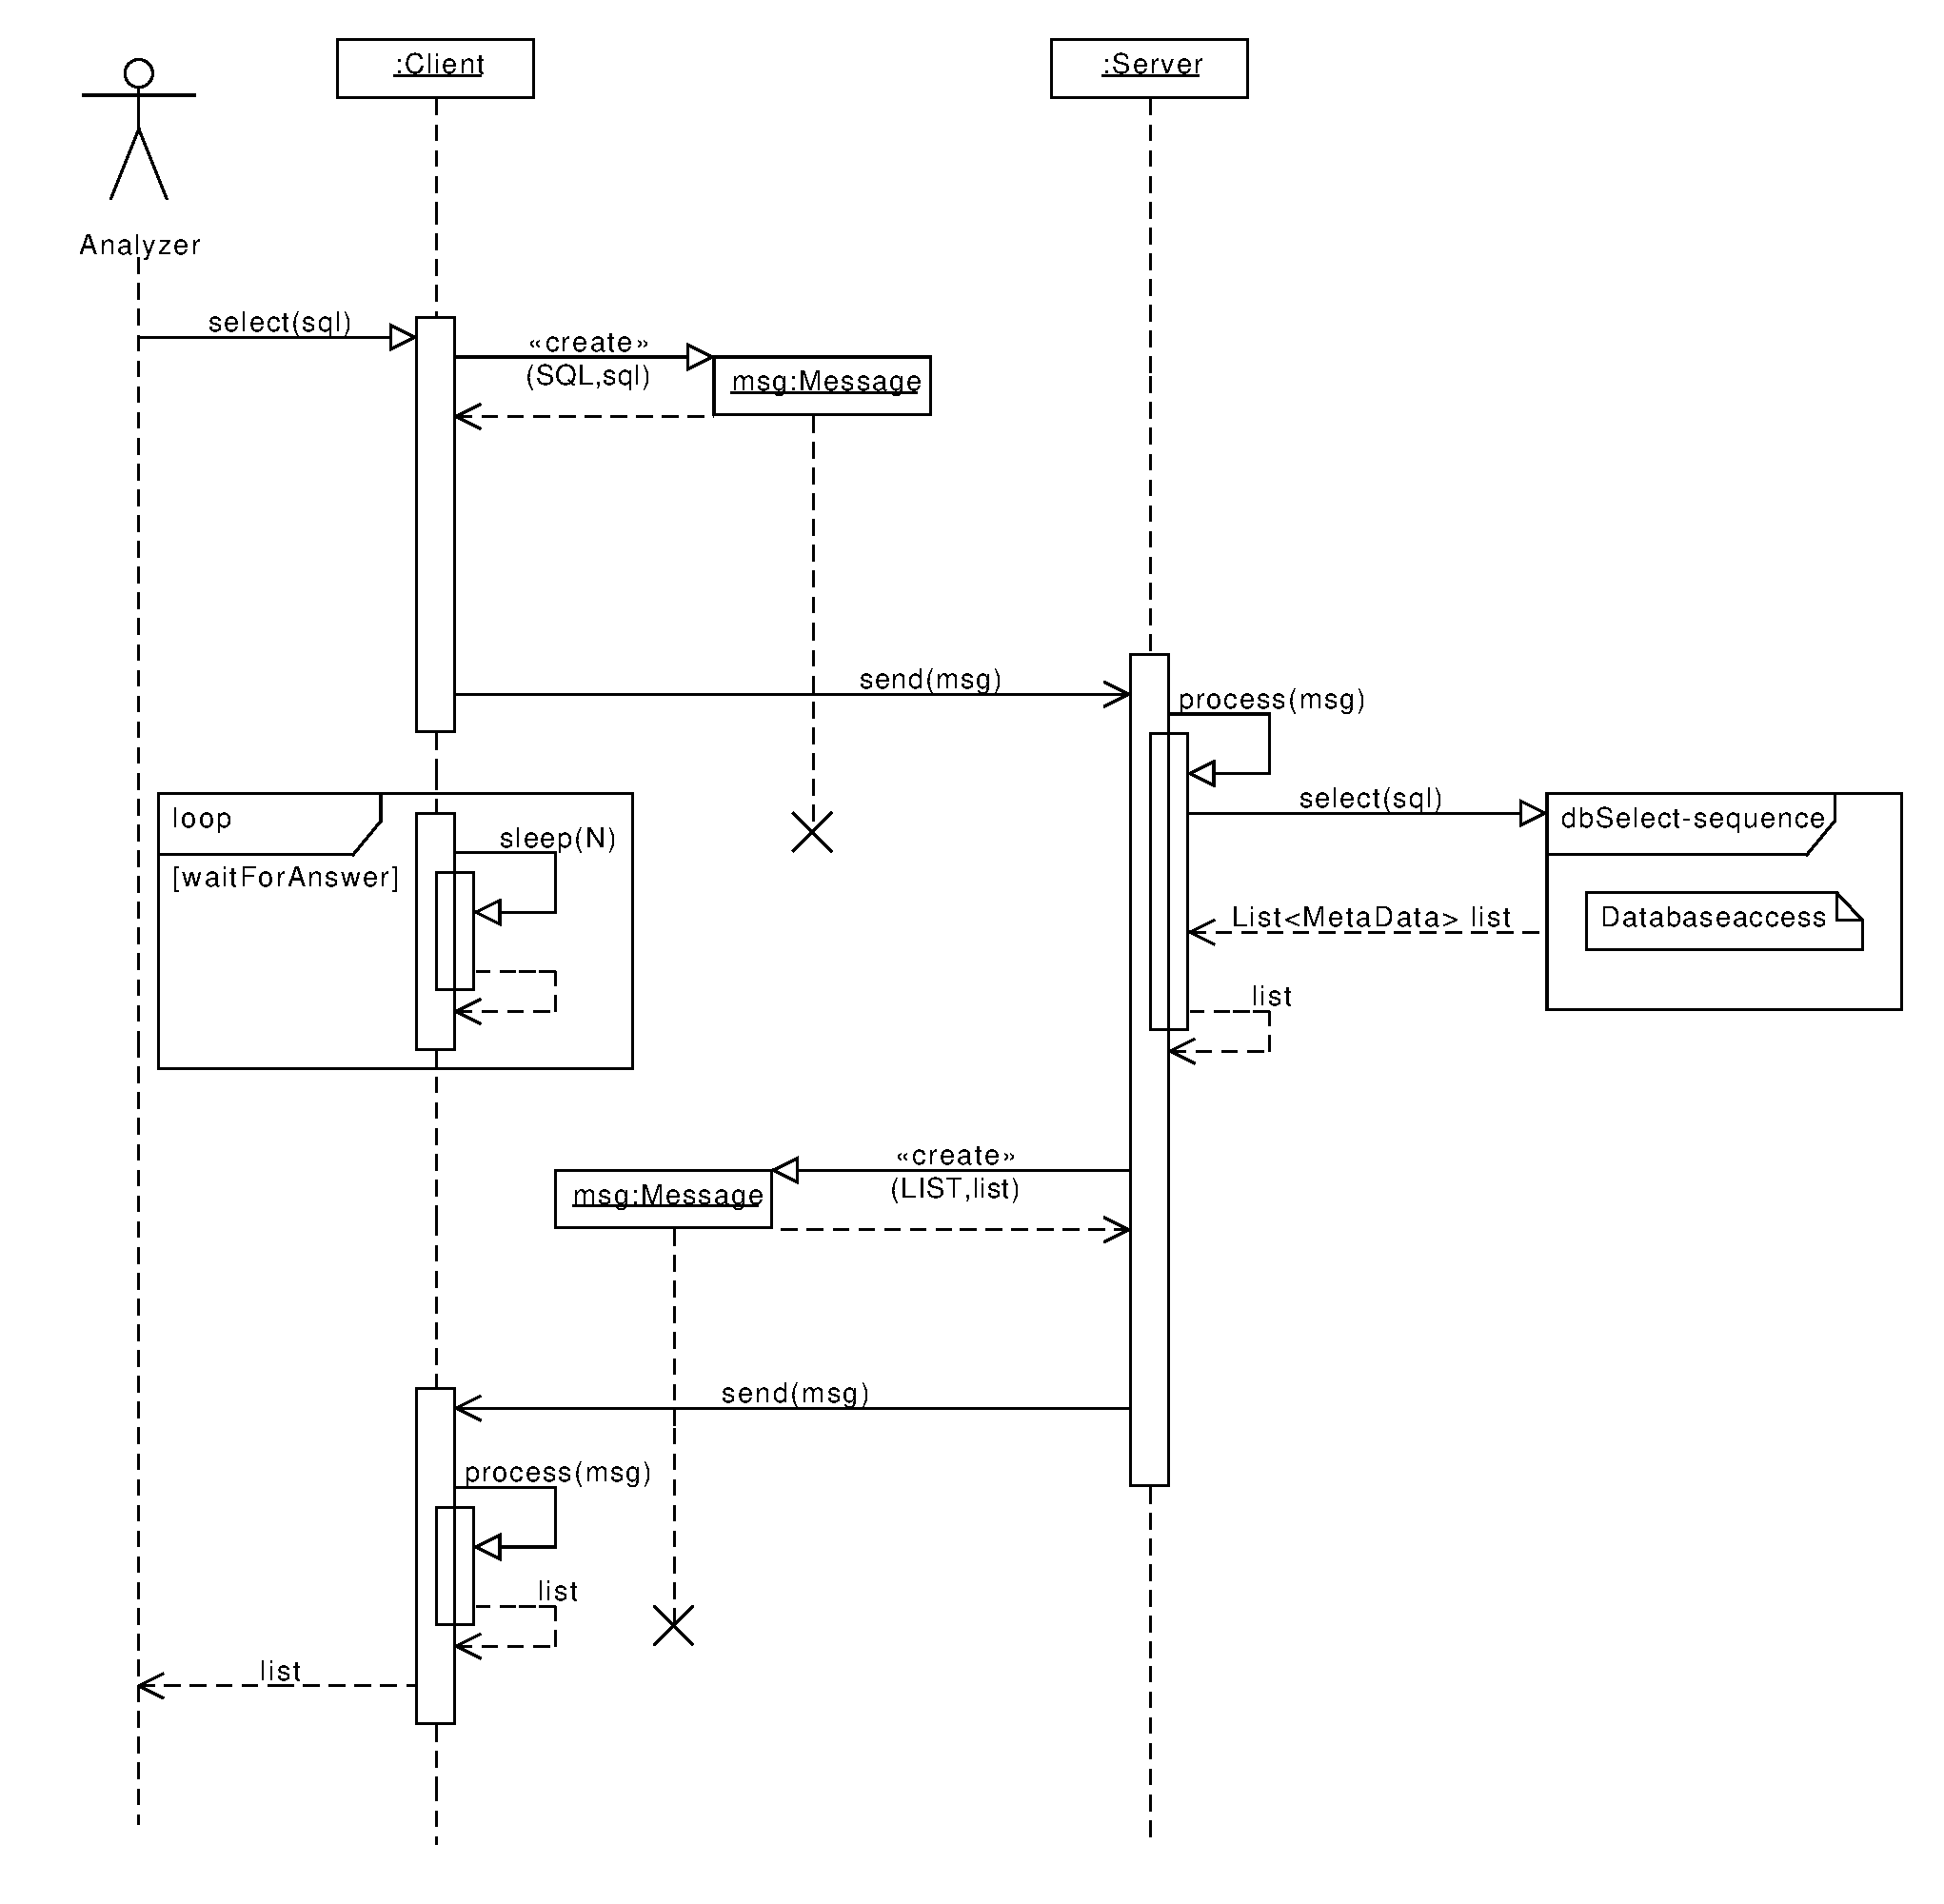
\includegraphics[width=\textwidth]{design/frontend/sequence/select-sequence.pdf}
%	\caption{Sequenzdiagramm: Select}
%\end{figure}

\subsection {add / deleteObserver}
\todo{sequence: addObserver}
%\begin{figure}[h]
%	\centering
%	\label{design:dia:sqc:select}
%	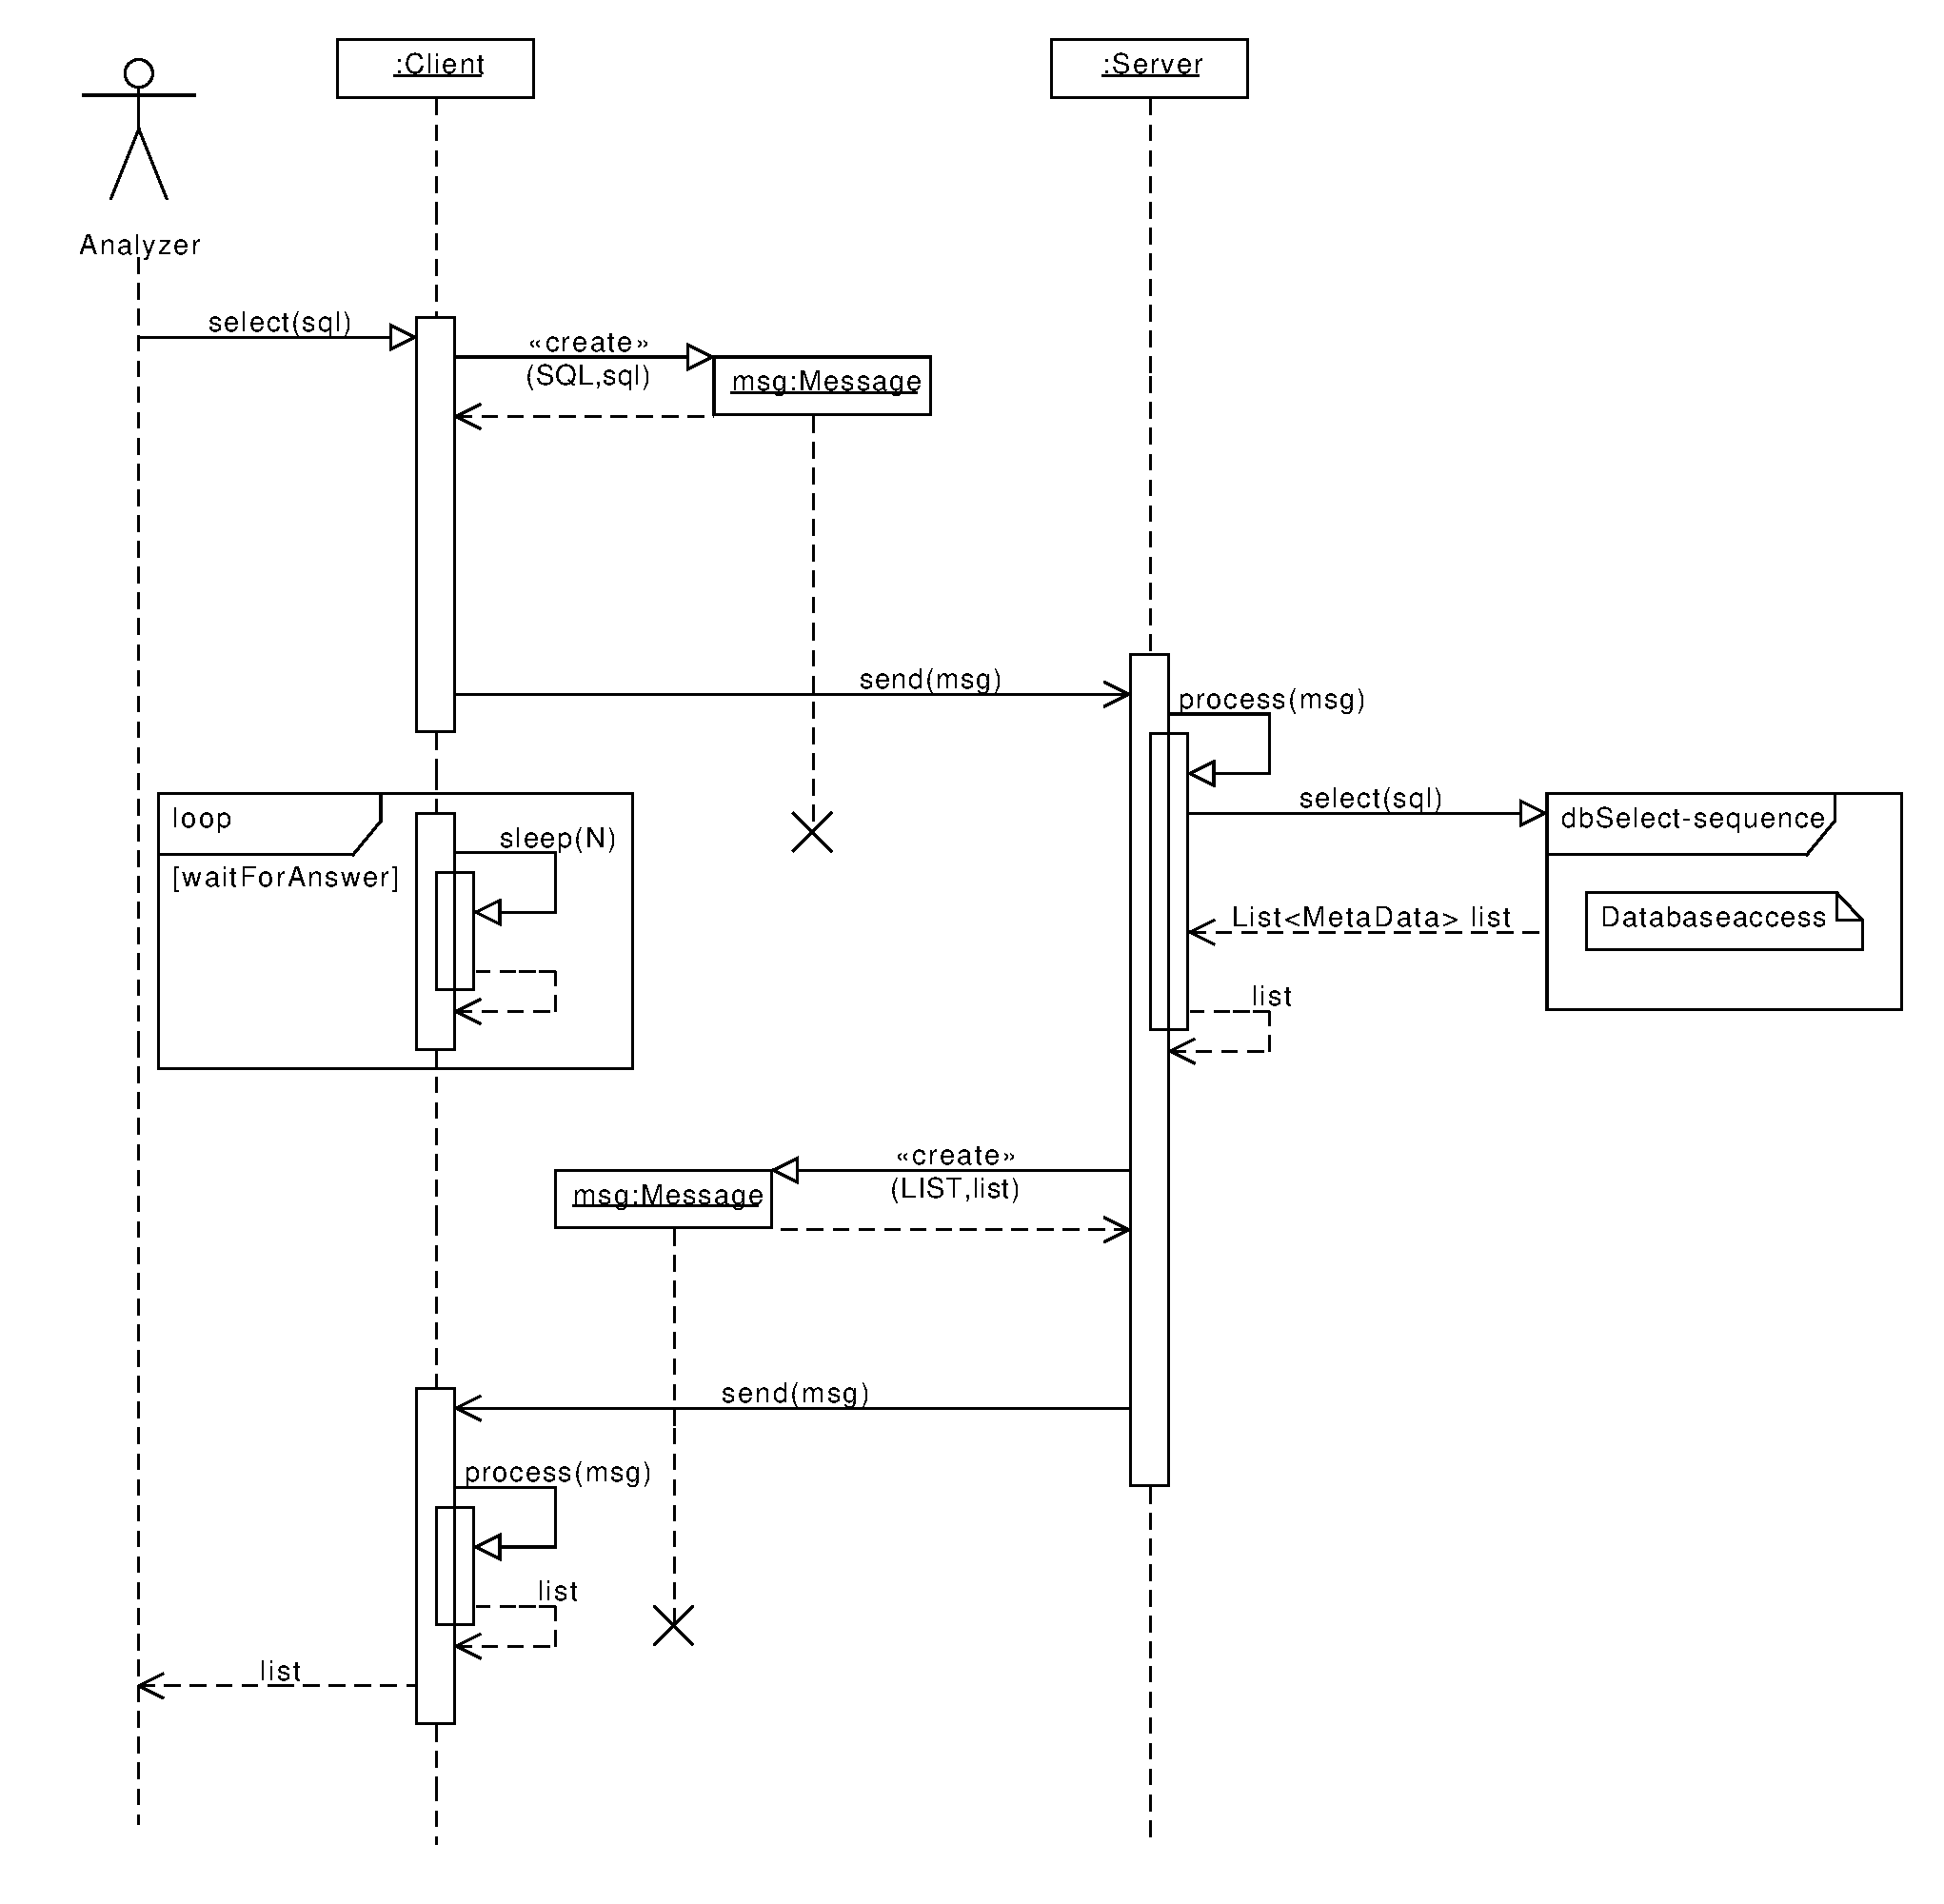
\includegraphics[width=\textwidth]{design/frontend/sequence/select-sequence.pdf}
%	\caption{Sequenzdiagramm: Select}
%\end{figure}

\subsection {notifyClients}
\todo{sequence: notifyClients}
%\begin{figure}[h]
%	\centering
%	\label{design:dia:sqc:select}
%	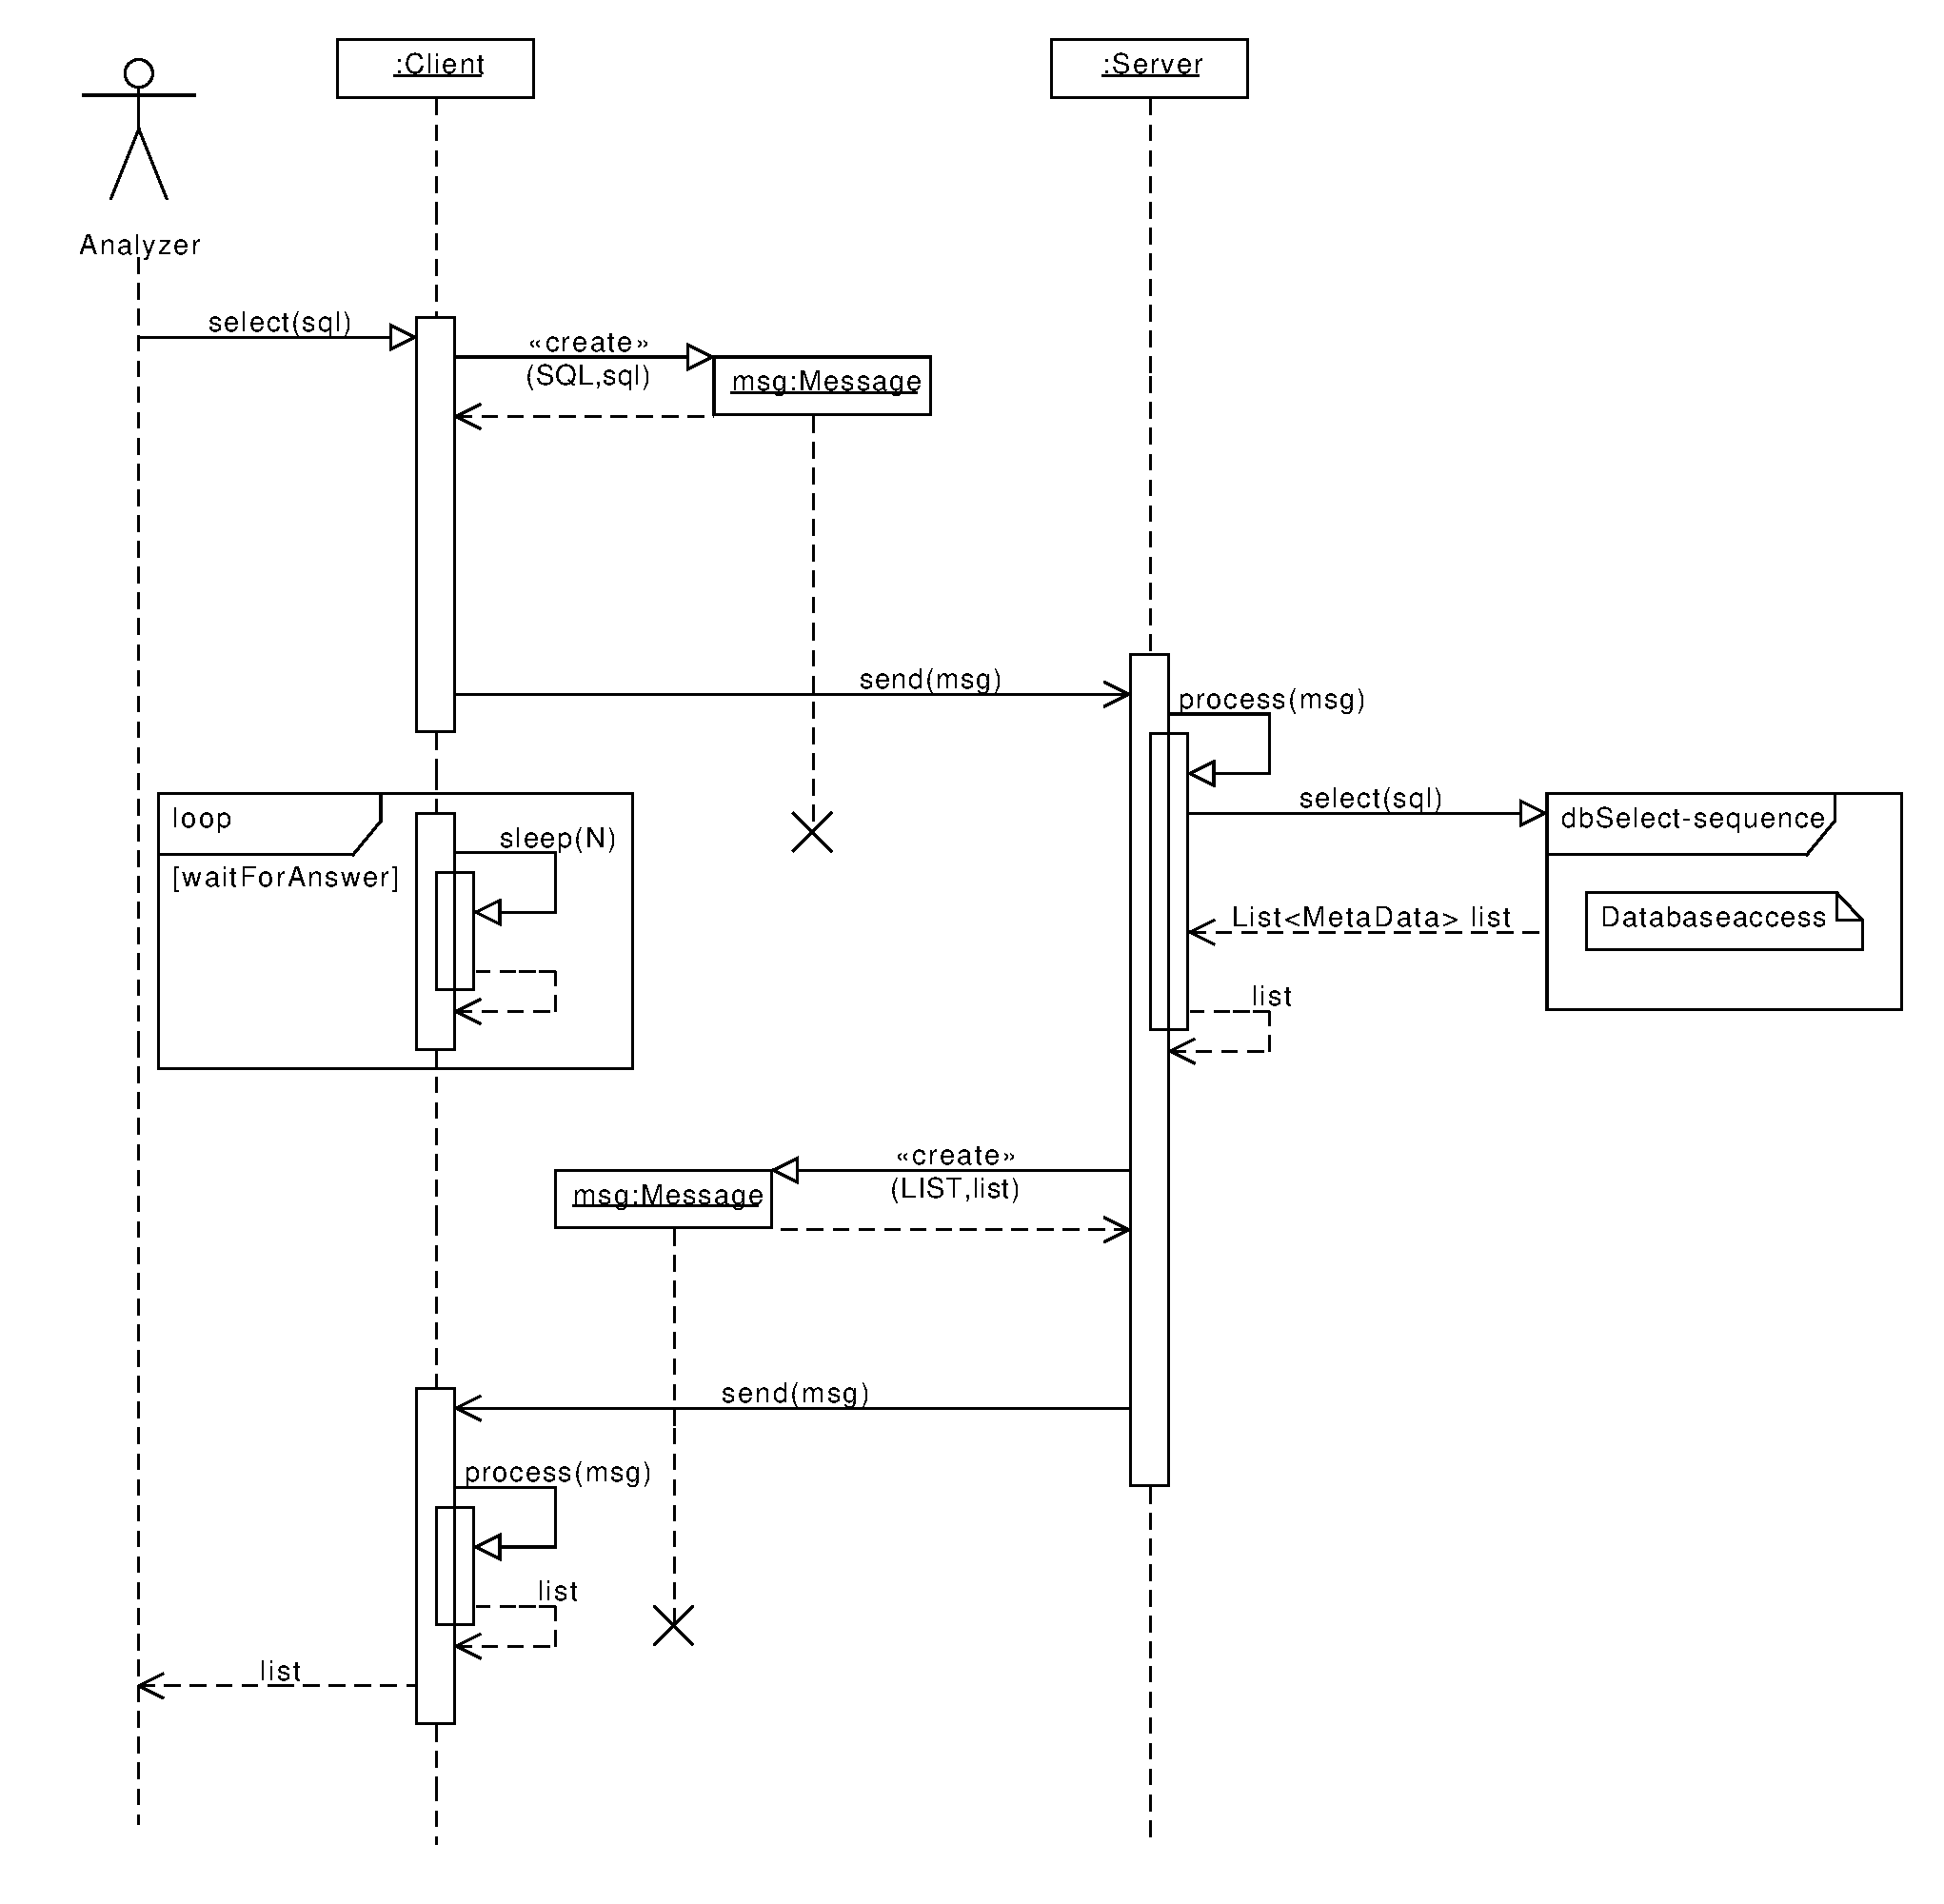
\includegraphics[width=\textwidth]{design/frontend/sequence/select-sequence.pdf}
%	\caption{Sequenzdiagramm: Select}
%\end{figure}

\section{Klassen und Komponenten}
